\documentclass[UTF8]{ctexart} % use larger type; default would be 10pt

\usepackage[utf8]{inputenc} % set input encoding (not needed with XeLaTeX)

%%% Examples of Article customizations
% These packages are optional, depending whether you want the features they provide.
% See the LaTeX Companion or other references for full information.

%%% PAGE DIMENSIONS
\usepackage{geometry} % to change the page dimensions
\geometry{a4paper} % or letterpaper (US) or a5paper or....
% \geometry{margin=2in} % for example, change the margins to 2 inches all round
% \geometry{landscape} % set up the page for landscape
%   read geometry.pdf for detailed page layout information

\usepackage{graphicx} % support the \includegraphics command and options

% \usepackage[parfill]{parskip} % Activate to begin paragraphs with an empty line rather than an indent

%%% PACKAGES
\usepackage{booktabs} % for much better looking tables
\usepackage{array} % for better arrays (eg matrices) in maths
\usepackage{paralist} % very flexible & customisable lists (eg. enumerate/itemize, etc.)
\usepackage{verbatim} % adds environment for commenting out blocks of text & for better verbatim
\usepackage{subfig} % make it possible to include more than one captioned figure/table in a single float
% These packages are all incorporated in the memoir class to one degree or another...

%%% HEADERS & FOOTERS
\usepackage{fancyhdr} % This should be set AFTER setting up the page geometry
\pagestyle{fancy} % options: empty , plain , fancy
\renewcommand{\headrulewidth}{0pt} % customise the layout...
\lhead{}\chead{}\rhead{}
\lfoot{}\cfoot{\thepage}\rfoot{}

%%% SECTION TITLE APPEARANCE
\usepackage{sectsty}
\allsectionsfont{\sffamily\mdseries\upshape} % (See the fntguide.pdf for font help)
% (This matches ConTeXt defaults)

%%% ToC (table of contents) APPEARANCE
\usepackage[nottoc,notlof,notlot]{tocbibind} % Put the bibliography in the ToC
\usepackage[titles,subfigure]{tocloft} % Alter the style of the Table of Contents
\renewcommand{\cftsecfont}{\rmfamily\mdseries\upshape}
\renewcommand{\cftsecpagefont}{\rmfamily\mdseries\upshape} % No bold!

%%% END Article customizations

%%% The "real" document content comes below...

\setlength{\parindent}{0pt}
\usepackage{physics}
\usepackage{amsmath}
%\usepackage{symbols}
\usepackage{amsfonts}
\usepackage{bm}
%\usepackage{eucal}
\usepackage{mathrsfs}
\usepackage{amssymb}
\usepackage{float}
\usepackage{multicol}
\usepackage{abstract}
\usepackage{empheq}
\usepackage{extarrows}


\DeclareMathOperator{\p}{\prime}
\DeclareMathOperator{\ti}{\times}
\DeclareMathOperator{\s}{\sum_{n=1}^{\infty}}
\DeclareMathOperator{\intinf}{\int_0^\infty}
\DeclareMathOperator{\intdinf}{\int_{-\infty}^\infty}
\DeclareMathOperator{\suminf}{\sum_{n=0}^\infty}
\DeclareMathOperator{\e}{\mathrm{e}}
\renewcommand{\I}{\mathrm{i}}
\DeclareMathOperator{\llra}{\longleftrightarrow}
\DeclareMathOperator{\lra}{\longrightarrow}
\DeclareMathOperator{\dlra}{\Leftrightarrow}
\DeclareMathOperator{\dra}{\Rightarrow}
\newcommand{\dis}{\displaystyle}
\numberwithin{equation}{section}

\title{Notes of GU Qiao MMP}
\author{hebrewsnabla}
%\date{} % Activate to display a given date or no date (if empty),
         % otherwise the current date is printed 

\begin{document}
% \boldmath
\maketitle


\section{Fundamental Conceptions}
\setcounter{subsection}{1}
\subsection{Vector Differential Operator \& Laplace Operator}
\subsubsection{Vector Differential Operator $\mathbf{\nabla}$}
\begin{equation}\label{key}
\nabla\equiv\pdv{x}\vb{i}+\pdv{y}\vb{j}+\pdv{z}\vb{k}
\end{equation}
def:\\
1) gradient of function $u$:\\
\begin{equation}\label{key}
\nabla u\equiv\pdv{u}{x}\vb{i}+\pdv{u}{y}\vb{j}+\pdv{u}{z}\vb{k}
\end{equation}
2) divergence of vector $\vb{E}$:\\
\begin{equation}\label{key}
\nabla\cdot \vb{E} \equiv \pdv{E_x}{x}+\pdv{E_y}{y}+\pdv{E_z}{z}
\end{equation}
3) curl of vector $\vb{E}$:\\
\begin{equation}\label{key}
\begin{aligned}
\nabla\times\vb{E} & \equiv
\mdet{\vb{i} & \vb{j} & \vb{k}\\
\dis\pdv{x} & \dis\pdv{y} & \dis\pdv{z}\\
E_x & E_y & E_z}\\
& = \qty(\pdv{E_z}{y}-\pdv{E_y}{z})\vb{i}+\qty(\pdv{E_x}{z}-\pdv{E_x}{z})\vb{j}+\qty(\pdv{E_y}{x}-\pdv{E_x}{y})\vb{k}
\end{aligned}
\end{equation}
Laplace Operator
\begin{equation}\label{key}
\ldots
\end{equation}
Relevant equations:\\
(4) \begin{equation}\label{key}
\nabla\cdot(u\vb{E})=(\nabla u)\cdot \vb{E}+u(\nabla\cdot \vb{E})
\end{equation}
(5) \begin{equation}\label{key}
\nabla\times(u\vb{E})=(\nabla u)\times\vb{E}+u(\nabla\times\vb{E})
\end{equation}
(6) \begin{equation}\label{key}
\nabla\cdot(\vb{E}\times\vb{F})=(\nabla\times\vb{E})\cdot\vb{F}-\vb{E}\cdot(\nabla\times\vb{F})
\end{equation}
Proof:
\begin{equation}\begin{aligned}
\nabla\cdot(\vb{E}\times\vb{F}) &=\qty(\pdv{x}\vb{i}+\pdv{y}\vb{j}+\pdv{z}\vb{k})\mdet{\vb{i} & \vb{j} & \vb{k}\\
	E_x & E_y & E_z\\
	F_x & F_y & F_z}\\
&=\pdv{x}(E_y F_z - E_z F_y)+\pdv{y}(E_z F_x - E_x F_z)+\pdv{z}(E_x F_y - E_y F_x)\\
& =\pdv{E_y}{x}F_z - \pdv{E_x}{z}F_y + \pdv{E_z}{y}F_x -\pdv{E_x}{y}F_z + \pdv{E_x}{z}F_y - \pdv{E_y}{z}F_x \\
&\quad + \pdv{F_z}{x}E_y -\pdv{F_y}{x}E_z + \pdv{F_x}{y}E_z -\pdv{F_z}{y}E_x + \pdv{F_y}{z}E_x - \pdv{F_x}{z}E_y\\
&=F_x(\pdv{E_z}{y} - \pdv{E_y}{z})+F_y(\pdv{E_x}{z} - \pdv{E_x}{z})+F_z(\pdv{E_y}{x} -\pdv{E_x}{y})\\
&\quad +E_x(\pdv{F_y}{z} -\pdv{F_z}{y})+E_y(\pdv{F_z}{x} - \pdv{F_x}{z})+E_z(\pdv{F_x}{y} -\pdv{F_y}{x})\\
&=(\nabla\times\vb{E})\cdot\vb{F}-\vb{E}\cdot(\nabla\times\vb{F})
\end{aligned}\end{equation}
(7) \begin{equation}\label{key}
\nabla\ti(\vb{E}\ti\vb{F})=(\vb{F}\cdot\nabla)\vb{E}-\vb{F}(\nabla\cdot\vb{E})-(\vb{E}\cdot\nabla)\vb{F}+\vb{E}(\nabla\cdot\vb{F})
\end{equation}
Proof:\\
(8) \begin{equation}\label{key}
\nabla (\vb{E}\cdot\vb{F}) = (\vb{F}\cdot\nabla)\vb{E}+(\vb{E}\cdot\nabla)\vb{F}+\vb{F}\ti(\nabla\ti\vb{E})+\vb{E}\ti(\nabla\ti\vb{F})
\end{equation}
Proof:\\
(9) \begin{equation}\label{key}
\nabla\ti(\nabla u)=0
\end{equation}
Proof:
\begin{equation}\label{key}
\begin{aligned}
\nabla\ti(\nabla u)
& =\nabla\ti(\pdv{u}{x}\vb{i}+\pdv{u}{y}\vb{j}+\pdv{u}{z}\vb{k})\\
& =\mdet{\vb{i} & \vb{j} & \vb{k}\\
	\dis\pdv{x} & \dis\pdv{y} & \dis\pdv{z}\\
	\dis\pdv{u}{x} & \dis\pdv{u}{y} & \dis\pdv{u}{z}}\\
& = 0
\end{aligned}
\end{equation}
(10) \begin{equation}\label{key}
\nabla\cdot(\nabla\ti\vb{E})=0
\end{equation}
Proof omitted.\\
(11) \begin{equation}\label{key}
\nabla\ti(\nabla\ti\vb{E})=\nabla(\nabla\cdot\vb{E})-\nabla^2\vb{E}
\end{equation}
Proof:\\
\subsubsection{Laplace Operator}
\paragraph{in polar coordinates}
\begin{equation}\label{key}
r=\sqrt{x^2+y^2}
\end{equation}
\begin{equation}\label{key}
\theta=\arctan{\dfrac{y}{x}}
\end{equation}
\begin{equation}\label{key}
\begin{aligned}
\pdv[2]{x} &=\pdv{x}\qty(\pdv{r}{x}\pdv{r}+\pdv{\theta}{x}\pdv{\theta})\\
&=\pdv[2]{r}{x}\pdv{r}+\pdv{r}{x}\qty(\pdv{r}{x}\qty(\pdv{r})^2+\pdv{\theta}{x}\pdv[2]{}{\theta}{r}) +\pdv[2]{\theta}{x}\pdv{\theta}+\pdv{\theta}{x}\qty(\pdv{r}{x}\pdv[2]{}{\theta}{r}+\pdv{\theta}{x}\qty(\pdv{\theta})^2)\\
&=\pdv[2]{r}{x}\pdv{r}+\pdv[2]{\theta}{x}\pdv{\theta}+\qty(\pdv{r}{x})^2\pdv[2]{r}+\qty(\pdv{\theta}{x})^2\pdv[2]{\theta}+2\pdv{r}{x}\pdv{\theta}{x}\pdv[2]{}{\theta}{r}
\end{aligned}
\end{equation}
while
\begin{equation}\label{key}
\pdv{r}{x}=\dfrac{x}{r}
\end{equation}
\begin{equation}\label{key}
\pdv[2]{r}{x}=\pdv{x}\dfrac{x}{r}=\dfrac{r-x\dfrac{x}{r}}{r^2}=\dfrac{y^2}{r^3}
\end{equation}
\begin{equation}\label{key}
\pdv{\theta}{x}=\dfrac{1}{1+\dfrac{y^2}{x^2}}\qty(-\dfrac{y}{x^2})=-\dfrac{y}{r^2}
\end{equation}
\begin{equation}\label{key}
\pdv[2]{\theta}{x}=2\dfrac{y}{r^3}\pdv{r}{x}=\dfrac{2xy}{r^4}
\end{equation}
Thus
\begin{equation}\label{key}
\pdv[2]{x}=\dfrac{y^2}{r^3}\pdv{r}+\dfrac{2xy}{r^4}\pdv{\theta}+\dfrac{x^2}{r^2}\pdv[2]{r}+\dfrac{y^2}{r^4}\pdv[2]{\theta}-\dfrac{2xy}{r^3}\pdv[2]{}{\theta}{r}
\end{equation}
In the same way
\begin{equation}\label{key}
\pdv[2]{y}=\dfrac{x^2}{r^3}\pdv{r}-\dfrac{2xy}{r^4}\pdv{\theta}+\dfrac{y^2}{r^2}\pdv[2]{r}+\dfrac{x^2}{r^4}\pdv[2]{\theta}+\dfrac{2xy}{r^3}\pdv[2]{}{\theta}{r}
\end{equation}
Thus
\begin{equation}\label{key}
\nabla^2=\pdv[2]{x}+\pdv[2]{y}=\dfrac{1}{r}\pdv{r}+\pdv[2]{r}+\dfrac{1}{r^2}\pdv[2]{\theta}
\end{equation}
More succinctly
\begin{equation}\label{key}
\nabla^2=\dfrac{1}{r}\pdv{r}\qty(r\pdv{r})+\dfrac{1}{r^2}\pdv[2]{\theta}
\end{equation}
\paragraph{in cylindrical coordinates}
\begin{equation}\label{key}
\nabla^2=\dfrac{1}{\rho}\pdv{\rho}\qty(\rho\pdv{\rho})+\dfrac{1}{\rho^2}\pdv[2]{\phi}+\pdv[2]{z}
\end{equation}
\paragraph{in spherical coordinates}
~\\
\begin{minipage}[H]{0.4\linewidth}
	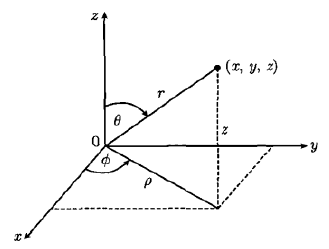
\includegraphics[width=\linewidth]{1.png}
\end{minipage}
\begin{minipage}[H]{0.6\linewidth}
	\begin{equation}\label{key}
	x=r\cos\phi\sin\theta
	\end{equation}
	\begin{equation}\label{key}
	y=r\sin\phi\sin\theta
	\end{equation}
	\begin{equation}\label{key}
	z=r\cos\theta
	\end{equation}
\end{minipage}
As mentioned above
\begin{equation}\label{key}
\rho=r\sin\theta,\;x=\rho\cos\phi,\;y=\rho\sin\phi
\end{equation}
\begin{equation}\label{1}
\pdv[2]{x}+\pdv[2]{y}=\pdv[2]{\rho}+\dfrac{1}{\rho}\pdv{\rho}+\dfrac{1}{\rho^2}\pdv[2]{\phi}
\end{equation}
Since
\begin{equation}\label{key}
z=r\cos\theta,\;\rho=r\sin\theta
\end{equation}
we have
\begin{equation}\label{2}
\pdv[2]{z}+\pdv[2]{\rho}=\pdv[2]{r}+\dfrac{1}{r}\pdv{r}+\dfrac{1}{r^2}\pdv[2]{\theta}
\end{equation}
According to $\eqref{1} \eqref{2}$,
\begin{equation}\label{key}
\begin{aligned}
\nabla^2 &=\pdv[2]{x}+\pdv[2]{y}+\pdv[2]{z}=\pdv[2]{r}+\dfrac{1}{r}\pdv{r}+\dfrac{1}{r^2}\pdv[2]{\theta}+\dfrac{1}{\rho}\pdv{\rho}+\dfrac{1}{\rho^2}\pdv[2]{\phi}\\
&=\pdv[2]{r}+\dfrac{1}{r}\pdv{r}+\dfrac{1}{r^2}\pdv[2]{\theta}+\dfrac{1}{r\sin\theta}\qty(\pdv{r}{\rho}\pdv{r}+\pdv{\theta}{\rho}\pdv{\theta})+\dfrac{1}{r^2 \sin^2\theta}\pdv[2]{\phi}
\end{aligned}
\end{equation}
$\because\; \dfrac{\rho}{z}=\tan\theta$\\
$\therefore$
\begin{equation}\label{key}
\pdv{\theta}{\rho}=\dfrac{1}{1+\dfrac{z^2}{\rho^2}}\dfrac{1}{z}=\dfrac{z}{r^2}=\dfrac{\cos\theta}{r}
\end{equation}
$\because\;\rho=r\sin\theta $\\
$\therefore$
\begin{equation}\label{key}
1=\pdv{r}{\rho}\sin\theta+r\cos\theta\pdv{\theta}{\rho}
\end{equation}
\begin{equation}\label{key}
\pdv{r}{\rho}=\sin\theta
\end{equation}
Thus
\begin{equation}\label{key}
\begin{aligned}
\nabla^2&=\pdv[2]{r}+\dfrac{1}{r}\pdv{r}+\dfrac{1}{r^2}\pdv[2]{\theta}+\dfrac{1}{r\sin\theta}\qty(\sin\theta\pdv{r}+\dfrac{\cos\theta}{r}\pdv{\theta})+\dfrac{1}{r^2 \sin^2\theta}\pdv[2]{\phi}\\
&=\pdv[2]{r}+\dfrac{2}{r}\pdv{r}+\dfrac{1}{r^2}\pdv[2]{\theta}+\dfrac{\cos\theta}{r^2\sin\theta}\pdv{\theta}+\dfrac{1}{r^2 \sin^2\theta}\pdv[2]{\phi}\\
&=\dfrac{1}{r^2}\pdv{r}\qty(r^2 \pdv{r})+\dfrac{1}{r^2 \sin{\theta}}\pdv{\theta}\qty(\sin\theta\pdv{\theta})+\dfrac{1}{r^2 \sin^2\theta}\pdv[2]{\phi}
\end{aligned}
\end{equation}


\section{Fourier Series}
\subsection{Fourier Series of Periodic Functions}
\begin{equation}\label{key}
f(x)=a_0+\sum_{n=1}^\infty(a_n\cos \dfrac{n\pi}{l}x+b_n\sin \dfrac{n\pi}{l}x)
\end{equation}
\begin{equation}\label{key}
a_0=\dfrac{1}{2l}\int_{-l}^{l}f(t)\dd{t}
\end{equation}
\begin{equation}\label{key}
a_n=\dfrac{1}{l}\int_{-l}^{l}f(t)\cos\dfrac{n\pi}{l}t\dd t
\end{equation}
\begin{equation}\label{key}
b_n=\dfrac{1}{l}\int_{-l}^{l}f(t)\sin\dfrac{n\pi}{l}t\dd t
\end{equation}
Discussion:
\begin{equation}\label{key}
\sum_{n=1}^\infty\dfrac{\sin nx}{n}=\dfrac{1}{2}(\pi-x)\quad(0<x<2\pi)
\end{equation}
WSJ:\\
\paragraph{Bessel Inequality}
\begin{equation}\label{key}
\abs{f(x)}^2 \geq a_0^2 + \sum_{k=1}^n a_k^2\cos \abs{\dfrac{k\pi}{l}x}^2 + \sum_{k=1}^n b_k\abs{\sin \dfrac{k\pi}{l}x}^2
\end{equation}
...
\paragraph{Parseval Equality}
\paragraph{Dirichlet Theorem}

\subsection{Half-range Fourier Series}
半幅傅里叶级数\\
For $0<x<l$\\
sine expansion:
\begin{equation}\label{key}
\phi(x)=\s c_n \sin\dfrac{n\pi}{l}x
\end{equation}
\begin{equation}\label{key}
c_n=\dfrac{2}{l}\int_{0}^{l}\phi(t)\sin\dfrac{n\pi}{l}\dd t
\end{equation}
cosine expansion:
\begin{equation}\label{key}
\phi(x)=d_0+ \s d_n \cos\dfrac{n\pi}{l}x
\end{equation}
\begin{equation}\label{key}
d_0=\dfrac{2}{l}\int_{0}^{l}\phi(t)\dd t
\end{equation}
\begin{equation}\label{key}
d_n=\dfrac{2}{l}\int_{0}^{l}\phi(t)\cos\dfrac{n\pi}{l}\dd t
\end{equation}
variants:
\begin{equation}\label{key}
\phi(x)=\s c_n^{\p} \sin\dfrac{(2n+1)\pi}{2l}x
\end{equation}
\begin{equation}\label{key}
\phi(x)=\s d_n^{\p} \cos\dfrac{(2n+1)\pi}{2l}x
\end{equation}
where
\begin{equation}\label{key}
c_n^{\p} =\int_0^l \phi(t)\sin\dfrac{(2n+1)\pi}{2l}t\dd t
\end{equation}
\begin{equation}\label{key}
d_n^{\p} =\int_0^l \phi(t)\cos\dfrac{(2n+1)\pi}{2l}t\dd t
\end{equation}

WSJ:\\
\paragraph{奇延拓,偶延拓}
\paragraph{Complex Fourier Expansion}
...\\
\subsection{Fourier Integral}
$f(x)$ is absolutely integrable in $(-\infty,\infty) \quad \Leftrightarrow  \quad \dis\int_{-\infty}^\infty \abs{f(x)}\dd x < \infty$\\
$$\Rightarrow \quad f(x)\rightarrow 0 \quad\text{when}\quad x\rightarrow\pm\infty$$
Consider an absolutely integrable periodic function with period $l$, whose Fourier series is
\begin{equation}\label{FS}
f(x)=a_0+\sum_{n=1}^\infty(a_n\cos \dfrac{n\pi}{l}x+b_n\sin \dfrac{n\pi}{l}x)
\end{equation}
\begin{equation}\label{key}
a_0=\dfrac{1}{2l}\int_{-l}^{l}f(t)\dd{t}
\end{equation}
\begin{equation}\label{key}
a_n=\dfrac{1}{l}\int_{-l}^{l}f(t)\cos\dfrac{n\pi}{l}t\dd t
\end{equation}
\begin{equation}\label{key}
b_n=\dfrac{1}{l}\int_{-l}^{l}f(t)\sin\dfrac{n\pi}{l}t\dd t
\end{equation}
To convert $f(x)$ to a non-periodic function in $(-\infty,\infty)$, we can let $l\rightarrow\infty$, thus
\begin{equation}\label{key}
a_0=\dfrac{1}{2l}\int_{-l}^{l}f(t)\dd{t}\rightarrow 0
\end{equation}
Moreover, we can let $\omega_n=\dfrac{n\pi}{l}$, thus
\begin{equation}\label{key}
\delta\omega=\omega_n - \omega_{n-1}=\dfrac{\pi}{l}\rightarrow 0
\end{equation}
so we can replace $\delta\omega$ with $\dd \omega$\\
i.e.
\begin{equation}\label{key}
\sum_{n=1}^\infty\cdots\Delta\omega\xrightarrow{l\rightarrow\infty}\int_0^\infty\cdots\dd \omega
\end{equation}
thus
\begin{equation}\label{key}
\begin{aligned}
\sum_{n=1}^\infty a_n\cos \dfrac{n\pi}{l}x &=\sum_{n=1}^\infty \dfrac{1}{l}\left[\int_{-l}^l f(t)\cos\dfrac{n\pi}{l}t\dd t\right]\cos\dfrac{n\pi}{l}x\\
&=\sum_{n=1}^\infty \dfrac{\Delta\omega}{\pi}\left[\int_{-l}^l f(t)\cos\omega_n t\dd t\right]\cos\omega_n x\\
&\xrightarrow{l\rightarrow\infty}\int_0^\infty \dd \omega \left[\dfrac{1}{\pi}\int_{-\infty}^\infty f(t)\cos\omega t \dd t\right]\cos\omega x
\end{aligned}
\end{equation}
\begin{equation}\label{key}
\sum_{n=1}^\infty a_n\sin \dfrac{n\pi}{l}x \xrightarrow{l\rightarrow\infty}\int_0^\infty \dd \omega \left[\dfrac{1}{\pi}\int_{-\infty}^\infty f(t)\sin\omega t \dd t\right]\sin\omega x
\end{equation}
Now we can rewrite $\eqref{FS}$ as Fourier integral expression
\begin{equation}\label{key}
f(x)=\int_0^\infty[A(\omega)\cos\omega x+B(\omega)\sin\omega x]\dd \omega
\end{equation}
where
\begin{equation}\label{key}
A(\omega)=\dfrac{1}{\pi}\int_{-\infty}^\infty f(t)\cos\omega t \dd t
\end{equation}
\begin{equation}\label{key}
B(\omega)=\dfrac{1}{\pi}\int_{-\infty}^\infty f(t)\sin\omega t \dd t
\end{equation}

\paragraph{Fourier Integral Theorem}
...\\

Discussion WSJ:\\
1) Fourier Integral can be rewritten as
\begin{equation}\label{key}
f(x) = \intinf C(\omega)\cos [\omega x - \phi(\omega)]\dd\omega
\end{equation}
where
\begin{equation}\label{key}
C(\omega) = \sqrt{A^2(\omega) + B^2(\omega)}
\end{equation}
\begin{equation}\label{key}
\phi(\omega) = \arctan\dfrac{B(\omega)}{A(\omega)}
\end{equation}
2) for odd functions\\
...\\
3) symmetrical Fourier Transform pair
\section{Fourier Transformation}
Def: \textbf{Integral transform} is to convert function $f(t)$ to $F(\beta)$ by integral calculation
\begin{equation}\label{key}
F(\beta)=\int_a^b f(t)K(\beta,t)\dd t
\end{equation}
where $K(\beta,t)$ is called kernel function or nucleus.
\subsection{Introduction}
\subsubsection{definition of FT}
Consider function $f(x)$ defined in $(-\infty,\infty)$, whose Fourier integral is
\begin{equation}\label{key}
\begin{aligned}
f(x) &=\int_0^\infty[A(\omega)\cos\omega x+B(\omega)\sin\omega x]\dd \omega\\
&=\dfrac{1}{\pi}\int_0^\infty\left(\int_{-\infty}^\infty f(t)(\cos\omega t\cos\omega x + \sin\omega t\sin\omega x)\dd t\right)\dd \omega\\
&=\dfrac{1}{\pi}\int_0^\infty\left(\int_{-\infty}^\infty f(t)\cos\omega (x-t) \dd t\right)\dd \omega\\
&=\dfrac{1}{2\pi}\int_0^\infty\left[\int_{-\infty}^\infty f(t)(\e^{\I\omega (x-t)}+\e^{-\I\omega (x-t)}) \dd t\right]\dd \omega\\
&=\dfrac{1}{2\pi}\int_{-\infty}^\infty\left[\int_0^\infty f(t)(\e^{\I\omega (x-t)}+\e^{-\I\omega (x-t)}) \dd \omega\right]\dd t
\end{aligned}
\end{equation}
Considering
\begin{equation}\label{key}
\int_0^\infty f(t)\e^{-\I\omega (x-t)} \dd \omega=\int_{-\infty}^0 f(t)\e^{\I\omega(x-t)}\dd \omega
\end{equation}
we have
\begin{equation}\label{key}
\begin{aligned}
f(x) &=\dfrac{1}{2\pi}\int_{-\infty}^\infty\left[\int_{-\infty}^\infty f(t)\e^{\I\omega (x-t)}\dd \omega\right]\dd t\\
&=\dfrac{1}{2\pi}\int_{-\infty}^\infty\left[\int_{-\infty}^\infty f(t)\e^{-\I\omega t} \dd t\right]\e^{\I\omega x}\dd \omega\\
&\equiv \dfrac{1}{2\pi}\int_{-\infty}^\infty F(\omega)\e^{i\omega x}\dd \omega
\end{aligned}
\end{equation}
i.e.
\begin{empheq}[box=\fbox]{align}
\label{FT}
F(\omega)&=\int_{-\infty}^\infty f(x)\e^{-\I\omega x} \dd x\\
\label{iFT}
f(x)&=\dfrac{1}{2\pi}\int_{-\infty}^\infty F(\omega)\e^{\I\omega x} \dd \omega
\end{empheq}
$F(\omega)$ is defined as a Fourier transform of $f(x)$, and $f(x)$ is defined as an inverse Fourier transform of $F(\omega)$, i.e.
\begin{equation}\label{Ftrans}
F(\omega)=\mathcal{F}\{f(x)\}
\end{equation}
\begin{equation}\label{key}
f(x)=\mathcal{F}^{-1}\{F(\omega)\}
\end{equation}
or
\begin{equation}\label{key}
F(\omega)\longleftrightarrow f(x)
\end{equation}
In $\eqref{Ftrans}$, $F(\omega)$ is called 象函数, $f(x)$ is called 原函数.\\
The process from $f(x)$ to $F(\omega)$ is called Fourier analysis. The inverse process is called 反演.\\
Discussion:\\
In $\eqref{FT}$, let $\omega=0$, we have
\begin{equation}\label{key}
F(0)=\intdinf f(x)\dd x
\end{equation}
In $\eqref{iFT}$, let $x=0$, we have
\begin{equation}\label{key}
f(0)==\dfrac{1}{2\pi}\intdinf F(\omega) \dd \omega
\end{equation}
\subsubsection{Features of FT}
1) Linear\\
$\cdots$\\
If $f(x)\llra F(\omega)$, we have the following theorems\\
2) Differential Theorem I\\
\begin{equation}\label{key}
\dv{f(x)}{x}\longleftrightarrow \I\omega F(\omega)
\end{equation}
Proof:\\
\begin{equation}\label{key}
\begin{aligned}
\dv{f(x)}{x}\longleftrightarrow\intdinf\dv{f(x)}{x}\e^{-\I\omega x}\dd x
&=\intdinf \dd f(x) \e^{-\I\omega x}\\
&=\left[f(x)\e^{-\I\omega x}\right]_{-\infty}^\infty + \I\omega\intdinf f(x) \e^{-\I\omega x}\dd x\\
&=\I\omega F(\omega)
\end{aligned}
\end{equation}
Likewise
\begin{equation}\label{key}
\qty(\dv{x})^n f(x)\llra (\I\omega)^n F(\omega)
\end{equation}
3) Differential Theorem II\\
\begin{equation}\label{key}
x f(x)\llra \I\dv{\omega}F(\omega)
\end{equation}
Proof:\\
\begin{equation}\label{key}
\begin{aligned}
\dv{\omega}F(\omega) &=\dv{\omega}\intdinf f(x)\e^{-\I\omega x}\dd{x}\\
&=\intdinf f(x)\dv{\omega}(\e^{-\I\omega x})\dd{x}\\
&=-\I\intdinf xf(x)\e^{-\I\omega x}\dd{x}\\
&=-\I\mathcal{F}\{xf(x)\}
\end{aligned}
\end{equation}
Likewise
\begin{equation}\label{key}
x^n f(x)\llra \I^n \qty(\dv{\omega})^n F(\omega)
\end{equation}
4) Integral Theorem\\
\begin{equation}\label{key}
\forall x_0,\; \int_{x_0}^x f(x)\dd{x}\llra\dfrac{F(\omega)}{\I\omega}
\end{equation}
5) Displacement Theorem\\
\begin{equation}\label{key}
\forall \xi,\;f(x+\xi)\llra\e^{\I\omega\xi}F(\omega)
\end{equation}
Proof:\\
\begin{equation}\label{key}
\begin{aligned}
\intdinf f(x+\xi)\e^{-\I\omega x}\dd{x}&\xlongequal{y=x+\xi}\intdinf f(y)\e^{-\I\omega(y-\xi)}\dd{y}\\
&=\e^{\I\omega\xi}\intdinf f(y)\e^{-\I\omega y}\dd{y}\\
&=\e^{\I\omega\xi}F(\omega)
\end{aligned}
\end{equation}
6) Convolution (卷积) Theorem\\
Def:\\
$f_1(x),\;f_2(x)$ defined at $(-\infty,\infty)$\\
Their convolution is defined as\\
\begin{equation}\label{key}
f_1(x)*f_2(x)=\intdinf f_1(\xi)f_2(x-\xi)\dd{\xi}
\end{equation}
Convolution Theorem:\\
\begin{equation}\label{key}
f_1(x)*f_2(x)\llra F_1(\omega)F_2(\omega)
\end{equation}
Proof:\\
\begin{equation}\label{key}
\begin{aligned}
\mathcal{F}\{f_1(x)*f_2(x)\}&=\intdinf f_1(x)*f_2(x)\e^{-\I\omega x}\dd x\\
&=\intdinf\left[\intdinf f_1(\xi)f_2(x-\xi)\dd{\xi}\right]\e^{-\I\omega x}\dd x\\
&=\intdinf f_1(\xi)\left[\intdinf f_2(x-\xi)\e^{-\I\omega (x-\xi)}\dd x\right]\e^{-\I\omega\xi}\dd{\xi}\\
&=\intdinf f_1(\xi)F_2(\omega)\e^{-\I\omega\xi}\dd{\xi}\\
&=F_2(\omega)\intdinf f_1(\xi)\e^{-\I\omega\xi}\dd{\xi}\\
&=F_1(\omega)F_2(\omega)
\end{aligned}
\end{equation}
$\therefore$
\begin{equation}\label{key}
f_1(x)*f_2(x)\llra F_1(\omega)F_2(\omega)
\end{equation}
Discussion:\\
6.1) Commutative property
\begin{equation}\label{key}
f_1(x)*f_2(x)=f_2(x)*f_1(x)
\end{equation}
6.2) For even fxn:
\begin{equation}\label{key}
f(x)*\cos\omega x = F(\omega)\cos\omega x
\end{equation}
\begin{equation}\label{key}
f(x)*\sin\omega x = F(\omega)\sin\omega x
\end{equation}
For odd fxn:
\begin{equation}\label{key}
f(x)*\cos\omega x = \I F(\omega)\sin\omega x
\end{equation}
\begin{equation}\label{key}
f(x)*\sin\omega x = -\I F(\omega)\cos\omega x
\end{equation}
Proof:\\
For even fxn
\begin{equation}\label{key}
\begin{aligned}
f(x)*\cos\omega x &= \intdinf f(\xi)\cos\omega(x-\xi)\dd\xi\\
&=\intdinf f(\xi)\left(\cos\omega x\cos\omega\xi+\sin\omega x\sin\omega\xi\right)\dd\xi\\
&=\cos\omega x\intdinf f(\xi)\cos\omega\xi\dd\xi\\
&=\cos\omega x\intdinf f(\xi)\left(\cos\omega\xi-\I\sin\omega\xi\right)\dd\xi\\
&=\cos\omega x\intdinf f(\xi)\e^{-\I\omega\xi}\dd\xi\\
&=F(\omega)\cos\omega x
\end{aligned}
\end{equation}
$\cdots$\\

WSJ:\\
1) 相似性定理\\
2) 延迟定理\\
3) 位移定理\\

\subsubsection{n-D Fourier Integral}
...\\

\subsection{Dirac $\delta$ Function}
\subsubsection{Definition}
\begin{equation}\label{key}
\delta(x-x_0)=\left\{
	\begin{array}{lr}
	0 & (x\neq x_0)\\
	\infty & (x=x_0)
	\end{array}
\right.
\end{equation}
\begin{equation}\label{key}
\intdinf\delta(x-x_0)\dd{x}=1
\end{equation}
Features:\\
WSJ:\\
阶跃函数:
\begin{equation}\label{key}
H(x) \equiv \left\{\mqty{0 &\quad x<0\\
						 1 &\quad x>0}\right.
	=\int_{-\infty}^x \delta(t)\dd t
\end{equation}
i.e. 
\begin{equation}\label{key}
\delta(x) = \dv{H(x)}{x}
\end{equation}
1) 筛选性质\\
$\forall$ continuous fxn $f(x)$,
\begin{equation}\label{key}
\intdinf f(x)\delta(x-x_0)\dd{x}=f(x_0)
\end{equation}
Proof:\\
\begin{equation}\label{key}
\begin{aligned}
\intdinf f(x)\delta(x-x_0)\dd{x}
&\xlongequal{\varepsilon\rightarrow 0}
\int_{x_0-\varepsilon}^{x_0+\varepsilon}f(x)\delta(x-x_0)\dd{x}\\
&=f(x_0)\int_{x_0-\varepsilon}^{x_0+\varepsilon}\delta(x-x_0)\dd{x}\\
&=f(x_0)
\end{aligned}
\end{equation}
\paragraph{Attention} 不是严格证明,不连续情况下不能用积分中值定理。\\
2) \\
\begin{equation}\label{key}
\delta(x)*f(x)=\intdinf f(\xi)\delta(x-\xi)\dd\xi=f(x)
\end{equation}
\begin{equation}\label{key}
\delta(x-a)*f(x)=\intdinf f(\xi)\delta(x-a-\xi)\dd\xi=f(x-a)
\end{equation}
\begin{equation}\label{key}
\delta(x-a)*\delta(x-b)=\delta(x-a-b)
\end{equation}
3) eigenfunction of operator $x$\\
\begin{equation}\label{key}
(x-x_0)\delta(x-x_0)=0
\end{equation}
\begin{equation}\label{key}
x\delta(x)=0
\end{equation}
正交归一性:
\begin{equation}\label{key}
\intdinf\delta(x-x_1)\delta(x-x_2)\dd{x}=\delta(x_1-x_2)
\end{equation}
完备性:
\begin{equation}\label{key}
f(x)=\intdinf f(\xi)\delta(\xi-x)\dd\xi
\end{equation}
4) FT of delta fxn\\
\begin{equation}\label{key}
\mathcal{F}\{\delta(x-x_0)\}=\intdinf\delta(x-x_0)\e^{-\I\omega x}\dd{x}=\e^{-\I\omega x_0}
\end{equation}
when $x_0=1$
\begin{equation}\label{key}
\mathcal{F}\{\delta(x)\}=1
\end{equation}
Thus
\begin{equation}\label{1}
\begin{aligned}
\delta(x)&=\dfrac{1}{2\pi}\intdinf\e^{\I\omega x}\dd\omega\\
&=\dfrac{1}{2\pi}\intdinf\e^{-\I\omega x}\dd\omega
\end{aligned}
\end{equation}
$\therefore$
\begin{equation}\label{key}
\delta(\omega)=\dfrac{1}{2\pi}\intdinf\e^{-\I\omega x}\dd x
\end{equation}
as a result
\begin{equation}\label{key}
\mathcal{F}\{\delta(x)\}=1
\end{equation}
\begin{equation}\label{key}
\mathcal{F}\{1\}=2\pi\delta(\omega)
\end{equation}
thus $1$ and $\delta(x)$ compose a Fourier transformation pair (傅里叶变换对).\\
Discussion:\\
1) \\
$\eqref{1}$ can be rewritten as
\begin{equation}\label{key}
\begin{aligned}
\delta(x)=&=\dfrac{1}{2\pi a}\intdinf\e^{-\tfrac{\I}{a}(a\omega) x}\dd(a\omega)\\
&\xlongequal{p=a\omega} \dfrac{1}{2\pi a}\intdinf\e^{-\tfrac{\I}{a}px}\dd{p}
\end{aligned}
\end{equation}
Let $x=p-p^{\p}$
\begin{equation}\label{key}
%\delta(p-p^{\p})=\dfrac{1}{2\pi a}\intdinf\e^
\end{equation}
2) momentum eigenfunction:
\begin{equation}\label{key}
\psi_p(x)=c\e^{\tfrac{\I}{\hbar}px}
\end{equation}
where
\begin{equation}\label{key}
c=\dfrac{1}{\sqrt{2\pi\hbar}}
\end{equation}
正交归一性:
\begin{equation}\label{key}
\begin{aligned}
\intdinf\psi_{p^{\p}}^{*} (x)\psi_p(x)\dd{x}
&=\abs{c}^2\intdinf\e^{\tfrac{\I}{\hbar}(p-p^{\p})}x\dd{x}\\
&=\abs{c}^2\cdot 2\pi\hbar\delta(p-p^{\p})\\
&=\delta(p-p^{\p})
\end{aligned}
\end{equation}
\section{Laplace Transformation}
f(t)不绝对可积\\
suppose
\begin{equation}\label{key}
g(t) = \e^{-\sigma t}f(t)H(t)
\end{equation}
\begin{equation}\label{key}
G(\omega) = \dfrac{1}{2\pi}\intdinf g(t)\e^{-\I\omega t}\dd t = \dfrac{1}{2\pi}\intinf f(t)\e^{-(\sigma+\I\omega)t}\dd t
\end{equation}
let $p=\sigma+\I\omega, \bar{f}(p) = 2\pi G(\omega)$, we have
\begin{equation}\label{key}
\bar{f}(p) = \intinf f(t)\e^{-pt}\dd t
\end{equation}
which is called Laplace Transformation.\\
Reverse L Transformation:
\begin{equation}\label{key}
f(t) = \dfrac{1}{2\pi\I}\int_{\sigma-\I\infty}^{\sigma+\I\infty} \bar{f}(p)\e^{pt}\dd p
\end{equation}
namely
\begin{empheq}[box=\fbox]{align}
\label{FT}
\mathcal{L}[f(t)] &= \bar{f}(p) = \intinf f(t)\e^{-pt}\dd t\\
\label{iFT}
\mathcal{L}^{-1}[\bar{f}(p)] &= f(t) = \dfrac{1}{2\pi\I}\int_{\sigma-\I\infty}^{\sigma+\I\infty} \bar{f}(p)\e^{pt}\dd p
\end{empheq}
Ex.
\begin{equation}\label{key}
\mathcal{L}[t]  = \dfrac{1}{p^2}
\end{equation}
\begin{equation}\label{key}
\mathcal{L}[\e^{st}] = \dfrac{1}{p-s}\quad\quad(\Re p>\Re s)
\end{equation}

\end{document}
